\chapter{Potentiel électrique~; conducteurs et condensateurs}\label{ch:b1:potential-capacitors}

Un champ, c'est trois nombres en chaque point~; un potentiel, c'en est un
seul. Parce que la force électrostatique est conservative, tout le champ d'une
distribution de charges se replie en une unique fonction scalaire, le
potentiel, d'où on le retrouve par dérivation --- la même économie qui, en
mécanique, avait changé les forces en \omterm{def:b1:work-and-energy:conservative}{énergie potentielle}. Le potentiel est ce
que lit un voltmètre, ce qu'entretient une pile, ce qui accélère les électrons
dans un tube~; ses surfaces de niveau donnent la carte d'un champ d'un coup
d'\omterm{def:b1:optical-instruments:eye}{œil}. Ce chapitre le construit, l'applique au dipôle (le premier modèle
électrique d'une molécule), puis passe aux deux objets dont tout circuit est
fait~: les conducteurs, sur lesquels les charges se disposent de façon à
annuler le champ intérieur, et les \omterm{def:b1:potential-capacitors:capacitance}{condensateurs}, qui stockent charge et
énergie dans un champ.

\begin{omfigure}
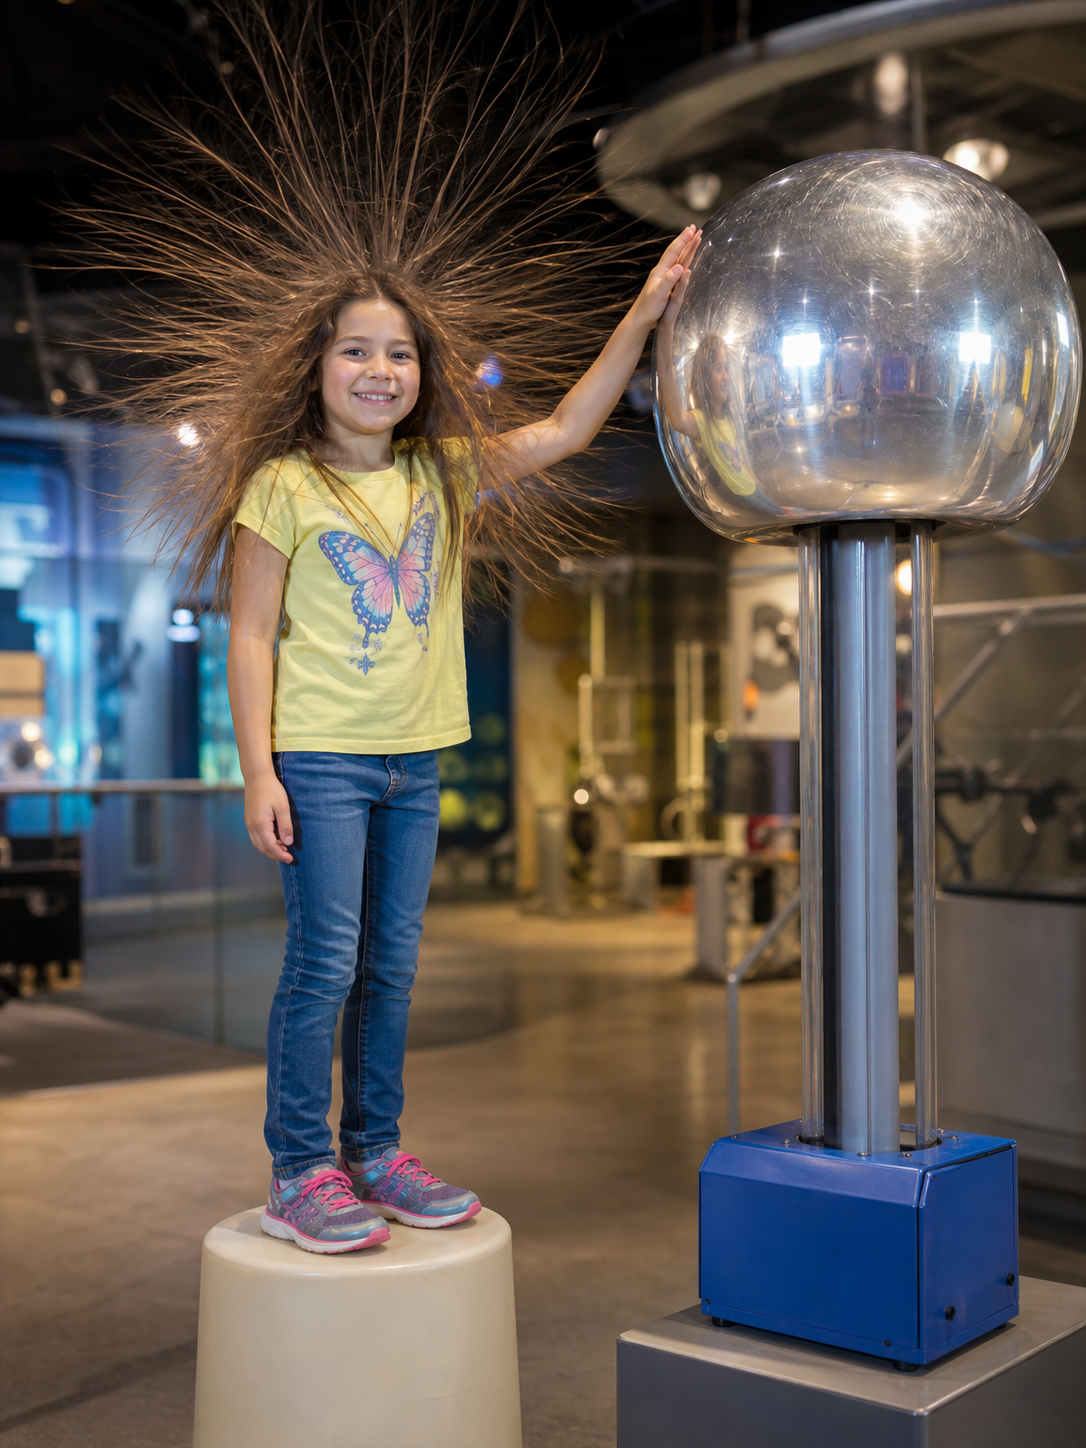
\includegraphics[width=0.34\linewidth]{images/book3/ai/b3-27-van-de-graaff-hair.png}

{\small Portée à quelques centaines de kilovolts par un générateur de Van de Graaff, une personne est un conducteur équipotentiel dont les cheveux, tous au même potentiel et tous chargés de même, se repoussent.}
\end{omfigure}

\section{Le potentiel électrostatique}

\begin{theorem}[Le champ électrostatique est conservatif]\label{thm:b1:potential-capacitors:potential}
\index{potentiel électrostatique}\index{volt}\index{circulation}
Il existe une fonction scalaire $V(M)$, le \emph{\omterm{thm:b1:potential-capacitors:potential}{potentiel
électrostatique}} (le volt, \unit{V}), telle que
\[
\vect E = -\overrightarrow{\operatorname{grad}}\,V , \qquad
V_A - V_B = \int_A^B \vect E\cdot\dd\vect l
\]
le long de tout chemin allant de $A$ à $B$ (la \emph{circulation} de $\vect E$
de $A$ à $B$ ne dépend pas du chemin, et elle est nulle sur un contour fermé).
Pour une charge ponctuelle $q$ en $O$, $V(M) = \dfrac{q}{4\pi\varepsilon_0\,OM}$
avec la convention $V(\infty) = 0$~; pour plusieurs charges, les potentiels
s'ajoutent. L'\omterm{def:b1:work-and-energy:conservative}{énergie potentielle} d'une charge $q'$ en $M$ vaut $E_p = q'V(M)$,
et le travail de la force électrique de $A$ à $B$ vaut $q'(V_A - V_B)$.
\end{theorem}

\begin{proof}
La force de Coulomb d'une charge fixe $q$ sur $q'$ a la forme de la
\omterm{def:b1:central-forces:gravitation}{gravitation} de Newton, avec $-Gm_1m_2$ remplacé par $qq'/4\pi\varepsilon_0$~; le
calcul même qui donnait $E_p = -Gm_1m_2/r$
(\cref{prop:b1:work-and-energy:eps}) donne $E_p = qq'/4\pi\varepsilon_0r$~: en
divisant par $q'$ on obtient $V$, et $\vect E = \vect F/q' =
-\overrightarrow{\operatorname{grad}}(E_p)/q'$. La superposition étend le
résultat à toute distribution~; la formule de circulation est la définition du
gradient intégrée le long du chemin.
\end{proof}

\begin{proposition}[Lire un potentiel]\label{prop:b1:potential-capacitors:reading}
\index{surface équipotentielle}
\begin{enumerate}
  \item Les \emph{\omterm{prop:b1:potential-capacitors:reading}{surfaces équipotentielles}} $V = \text{const}$ sont partout
        perpendiculaires aux \omterm{def:b1:electrostatics-gauss:field}{lignes de champ}, et le champ est dirigé vers les
        potentiels \emph{décroissants}.
  \item $|\vect E|$ est le taux de variation de $V$ selon la direction de plus
        grande pente~: là où les équipotentielles se resserrent, le champ est intense.
  \item $V$ n'est défini qu'à une constante additive près~; seules les
        différences (les tensions) sont mesurables. On prend par convention la
        terre ou l'infini comme origine.
  \item En \omterm{def:b1:point-kinematics:spherical}{coordonnées sphériques}, avec symétrie autour de $O$, $E_r = -\dd V/
        \dd r$~; en \omterm{def:b1:point-kinematics:cylindrical}{coordonnées polaires} $(r, \theta)$ dans un plan,
        $E_r = -\partial V/\partial r$ et $E_\theta = -\dfrac1r\,\partial V/\partial\theta$.
\end{enumerate}
\end{proposition}

\begin{proof}
Sur une équipotentielle, $\dd V = -\vect E\cdot\dd\vect l = 0$ pour tout
déplacement dans la surface, donc $\vect E$ lui est normal~; en se déplaçant
selon $\vect E$, $\dd V = -E\,\dd l < 0$. Les composantes polaires découlent de
$\dd V = (\partial V/\partial r)\dd r + (\partial V/\partial\theta)\dd\theta$ et de
$\dd\vect l = \dd r\,\vect e_r + r\,\dd\theta\,\vect e_\theta$.
\end{proof}

\begin{omfigure}
\begin{tikzpicture}[font=\small, x=1cm, y=1cm, >=Stealth]
  \begin{scope}
    \foreach \r in {0.6,0.85,1.2,1.7,2.4} \draw[omProp, thick] (0,0) circle (\r);
    \foreach \a in {0,30,...,330} \draw[omDef, ->] (0.25,0) ++({\a}:0) -- ++({\a}:2.7) ;
    \fill[omThm] (0,0) circle (2.5pt) node[below left, font=\footnotesize] {$q > 0$};
    \node[omProp, font=\footnotesize] at (2.05,2.05) {$V = \text{const}$};
    \node[font=\footnotesize] at (0,-3.1) {charge ponctuelle~: sphères $V \propto 1/r$};
  \end{scope}
  \begin{scope}[xshift=8.4cm]
    \draw[omThm, very thick] (-2.2,-2.2) -- (-2.2,2.2) node[above] {$V_1$};
    \draw[omDef, very thick] (2.2,-2.2) -- (2.2,2.2) node[above] {$V_2 < V_1$};
    \foreach \x in {-1.32,-0.44,0.44,1.32} \draw[omProp, thick] (\x,-2.0) -- (\x,2.0);
    \foreach \y in {-1.5,-0.5,0.5,1.5} \draw[omDef, ->] (-2.1,\y) -- (2.0,\y);
    \node[omProp, font=\footnotesize, anchor=west] at (-1.3,2.25) {équipotentielles};
    \node[font=\footnotesize] at (0,-3.1) {condensateur plan~: plans, $V$ linéaire en $x$};
  \end{scope}
\end{tikzpicture}

{\small Équipotentielles (en orange) et \omterm{def:b1:electrostatics-gauss:field}{lignes de champ} (en bleu) d'une charge
ponctuelle et d'un \omterm{prop:b1:potential-capacitors:three}{condensateur plan}. Les lignes coupent les équipotentielles
à angle droit et vont des potentiels élevés vers les faibles~; là où les
équipotentielles se resserrent, le champ est intense.}
\end{omfigure}

\begin{method}[Calculer un potentiel]\label{meth:b1:potential-capacitors:compute}
Ou bien l'on somme $\dd q/4\pi\varepsilon_0r$ sur la distribution (lorsque la somme
est calculable et la distribution finie, de sorte que $V(\infty) = 0$ ait un
sens), ou bien l'on intègre $\dd V = -\vect E\cdot\dd\vect l$ le long d'un
chemin commode à partir d'un point où $V$ est connu, en utilisant le champ
donné par le \omterm{thm:b1:electrostatics-gauss:gauss}{théorème de Gauss}. Pour les distributions infinies (fil, plan),
seule la seconde voie fonctionne, et l'origine de $V$ doit être choisie en un
point à distance finie.
\end{method}

\begin{proposition}[Potentiels des distributions classiques]\label{prop:b1:potential-capacitors:classic}
\begin{enumerate}
  \item Sphère de rayon $R$ portant $Q$ dans son volume~: $V(r) = \dfrac{Q}{4\pi\varepsilon_0r}$
        à l'extérieur~; $V(r) = \dfrac{Q}{4\pi\varepsilon_0}\,\dfrac{3R^2 - r^2}{2R^3}$
        à l'intérieur, de sorte que $V(0) = \tfrac32\,Q/4\pi\varepsilon_0R$. Si $Q$ est
        portée par la surface, $V$ est uniforme à l'intérieur et vaut $Q/4\pi\varepsilon_0R$.
  \item Fil infini de charge linéique $\lambda$~: $V(r) = -\dfrac{\lambda}{2\pi\varepsilon_0}\ln\dfrac{r}{r_0}$.
  \item \omterm{prop:b1:potential-capacitors:three}{Condensateur plan}, champ $E$ de l'armature~1 vers l'armature~2 distante
        de $d$~: $V$ décroît linéairement dans l'intervalle et $V_1 - V_2 = Ed$.
\end{enumerate}
\end{proposition}

\begin{proof}
On intègre $E_r = -\dd V/\dd r$ avec les champs de la
\cref{prop:b1:electrostatics-gauss:three}~: depuis l'infini vers l'intérieur
pour la sphère (la continuité en $R$ fixe la constante intérieure), depuis
$r_0$ pour le fil, à travers l'intervalle pour le \omterm{def:b1:potential-capacitors:capacitance}{condensateur}.
\end{proof}

\begin{omfigure}
\begin{tikzpicture}
\begin{axis}[omaxis, axis x line=bottom, axis y line=left, width=10cm, height=5.8cm,
    xlabel={$r/R$}, ylabel={},
    xlabel style={at={(axis description cs:0.5,-0.1)}, anchor=north},
    xmin=0, xmax=4, ymin=0, ymax=1.7, xtick={1,2,3}, ytick={0.5,1,1.5}, samples=80, clip=false]
  \addplot[omProp, very thick, domain=0:1] {1.5-0.5*x^2};
  \addplot[omProp, very thick, domain=1:4] {1/x};
  \node[omProp, font=\footnotesize, anchor=east] at (axis cs:3.95,1.5) {$V$ (en unités de $Q/4\pi\varepsilon_0R$)};
  \addplot[omDef, thick, dashed, domain=0:1] {x};
  \addplot[omDef, thick, dashed, domain=1:4] {1/x^2};
  \node[omDef, font=\footnotesize, anchor=east] at (axis cs:3.95,1.27) {$E$ (en unités de $Q/4\pi\varepsilon_0R^2$)};
  \node[omProp, font=\footnotesize, anchor=west] at (axis cs:0.05,1.58) {$V(0) = \tfrac32\,V(R)$};
\end{axis}
\end{tikzpicture}

{\small Potentiel (trait plein) et champ (pointillés) d'une sphère
uniformément chargée. Le potentiel est continu et de pente continue~; il est
parabolique à l'intérieur, où le champ est linéaire, et en $1/r$ à
l'extérieur. Son maximum est au centre, où le champ s'annule --- un maximum de
$V$ est un point de champ nul, et non l'inverse.}
\end{omfigure}

\begin{example}[L'électronvolt, à nouveau]\label{ex:b1:potential-capacitors:eV}
Un électron qui franchit un intervalle sous \qty{100}{V} gagne $eU = \qty{100}{eV} =
\qty{1.6e-17}{J}$, quelle que soit la forme du champ entre les électrodes~: le
potentiel rend le chemin indifférent
(\cref{def:b1:charged-particles:eV}). Une charge de \qty{1}{\micro C} à
\qty{1}{m} d'une autre est au potentiel $V = \qty{9}{kV}$ et le couple stocke
\qty{9}{mJ}~; le potentiel au centre d'un noyau d'or vaut
\qty{24}{MV} (\cref{exo:b1:potential-capacitors:6}).
\end{example}

\section{Le dipôle électrique}

\begin{definition}[Dipôle électrique]\label{def:b1:potential-capacitors:dipole}
\index{dipôle électrique}\index{moment dipolaire}
Deux charges opposées, $-q$ en $N$ et $+q$ en $P$, distantes de $a = NP$,
forment un \emph{dipôle électrique} de \emph{moment dipolaire}
$\vect p = q\,\vect{NP}$ (\unit{C.m}), dirigé du $-$ vers le $+$.
L'approximation dipolaire est l'étude de son champ aux distances $r \gg a$.
Une molécule dont les \omterm{def:b1:systems-of-points:cm}{barycentres} des charges positives et négatives ne
coïncident pas (l'eau, $p = \qty{6.2e-30}{C.m}$) est un dipôle~; un atome
neutre plongé dans un champ en devient un (dipôle induit).
\end{definition}

\begin{proposition}[Champ d'un dipôle]\label{prop:b1:potential-capacitors:dipolefield}
En $M$ avec $OM = r \gg a$ ($O$ le milieu de $NP$) et $\theta$ l'angle entre
$\vect p$ et $\vect{OM}$,
\[
V(M) = \frac{p\cos\theta}{4\pi\varepsilon_0 r^2}, \qquad
E_r = \frac{2p\cos\theta}{4\pi\varepsilon_0r^3}, \qquad
E_\theta = \frac{p\sin\theta}{4\pi\varepsilon_0r^3} .
\]
Le champ d'un dipôle décroît en $1/r^3$, plus vite que le
$1/r^2$ d'une charge~: de loin, les deux charges se compensent presque, et il
ne reste que leur écartement.
\end{proposition}

\begin{proof}
$V = \dfrac{q}{4\pi\varepsilon_0}\Bigl(\dfrac1{PM} - \dfrac1{NM}\Bigr)$ avec
$PM \approx r - \tfrac a2\cos\theta$ et $NM \approx r + \tfrac a2\cos\theta$
(projection de $\pm\tfrac a2$ sur $\vect{OM}$)~; au premier ordre en $a/r$,
$1/PM - 1/NM \approx a\cos\theta/r^2$. Puis $E_r = -\partial V/\partial r$ et
$E_\theta = -(1/r)\,\partial V/\partial\theta$.
\end{proof}

\begin{omfigure}
\begin{tikzpicture}[font=\small, x=1cm, y=1cm, >=Stealth]
  \begin{scope}[scale=1.3]
    \fill[omDef] (-0.5,0) circle (2.5pt) node[below left, font=\footnotesize] {$-q$};
    \fill[omThm] (0.5,0) circle (2.5pt) node[below right, font=\footnotesize] {$+q$};
    \draw[->, very thick] (-0.5,0) -- (0.5,0); \node[above, font=\footnotesize] at (0,0.05) {$\vect p$};
    \fill (0,0) circle (1pt); \node[below, font=\footnotesize] at (0,-0.05) {$O$};
    \coordinate (M) at (2.6,1.9);
    \fill (M) circle (1.6pt) node[above right, font=\footnotesize] {$M$};
    \draw[dashed] (0,0) -- (M) node[midway, above left, font=\footnotesize] {$r$};
    \draw[dashed] (-0.5,0) -- (M); \draw[dashed] (0.5,0) -- (M);
    \draw (0.9,0) arc[start angle=0, end angle=36, radius=0.9] node[midway, right, font=\footnotesize] {$\theta$};
    \draw[->, omThm, thick] (M) -- ++(36:0.9) node[right, font=\footnotesize] {$E_r$};
    \draw[->, omThm, thick] (M) -- ++(126:0.6) node[above left, font=\footnotesize] {$E_\theta$};
  \end{scope}
  \begin{scope}[xshift=8.6cm, scale=1.0]
    % field lines: circles through the charges (dipole limit: r = K sin^2 theta)
    \foreach \K in {0.8,1.6,2.6} {
      \draw[omDef, thick, domain=3:177, samples=60, smooth] plot ({\K*sin(\x)*sin(\x)*cos(\x)}, {\K*sin(\x)*sin(\x)*sin(\x)});
      \draw[omDef, thick, domain=183:357, samples=60, smooth] plot ({\K*sin(\x)*sin(\x)*cos(\x)}, {\K*sin(\x)*sin(\x)*sin(\x)});
    }
    % equipotentials r = A sqrt(|cos theta|)
    \foreach \A in {0.9,1.5,2.2} {
      \draw[omProp, thick, domain=-88:88, samples=50, smooth] plot ({\A*sqrt(cos(\x))*cos(\x)}, {\A*sqrt(cos(\x))*sin(\x)});
      \draw[omProp, thick, domain=92:268, samples=50, smooth] plot ({\A*sqrt(-cos(\x))*cos(\x)}, {\A*sqrt(-cos(\x))*sin(\x)});
    }
    \draw[->, very thick] (-0.25,0) -- (0.25,0);
    \node[font=\footnotesize, omProp] at (2.95,0.45) {$V > 0$};
    \node[font=\footnotesize, omProp] at (-2.95,0.45) {$V < 0$};
  \end{scope}
\end{tikzpicture}

{\small À gauche~: la géométrie de l'approximation dipolaire --- $M$ vu depuis
le centre $O$ à la distance $r$ et sous l'angle $\theta$ à partir de $\vect p$,
avec les composantes radiale et orthoradiale du champ. À droite~: \omterm{def:b1:electrostatics-gauss:field}{lignes de
champ} (en bleu, $r \propto \sin^2\theta$) et équipotentielles (en orange, $r \propto
\sqrt{|\cos\theta|}$) d'un dipôle dirigé vers la droite~; le plan passant par $O$
et perpendiculaire à $\vect p$ est l'équipotentielle $V = 0$.}
\end{omfigure}

\begin{proposition}[Dipôle dans un champ extérieur]\label{prop:b1:potential-capacitors:dipoleinfield}
\index{dipôle!moment des forces}\index{dipôle!énergie}
Un dipôle $\vect p$ placé dans un champ uniforme $\vect E$ ne subit aucune
force résultante, mais un moment $\vect\Gamma = \vect p\wedge\vect E$ qui tend
à l'aligner sur le champ, et il a l'\omterm{def:b1:work-and-energy:conservative}{énergie potentielle} $E_p = -\vect p\cdot\vect E$,
minimale lorsqu'il est aligné. Dans un champ non uniforme, il est en outre
attiré vers les régions de champ intense (à une dimension, $F_x = p\,\dd E/\dd x$
pour un dipôle aligné).
\end{proposition}

\begin{proof}
Les forces $\pm q\vect E$ se compensent~; leur moment en $O$ vaut $\vect{OP}\wedge
q\vect E + \vect{ON}\wedge(-q\vect E) = q\vect{NP}\wedge\vect E$. Énergie~:
$qV(P) - qV(N) = -q\,\vect{NP}\cdot\vect E$ pour un champ uniforme (puisque $V(P)
- V(N) = -\vect E\cdot\vect{NP}$). En champ non uniforme, aligné selon $x$~: $F_x =
qE(x + a) - qE(x) \approx qa\,\dd E/\dd x$.
\end{proof}

\begin{example}[Pourquoi le peigne attire le papier]\label{ex:b1:potential-capacitors:comb}
Un peigne chargé crée un champ qui décroît avec la distance~; un morceau de
papier, neutre, y est polarisé (dipôle induit selon $\vect E$), et la force
$p\,\dd E/\dd x$ sur un dipôle aligné l'attire vers la région de champ
intense~: le peigne. Le signe de la charge du peigne est indifférent~; le même
mécanisme colle le ballon au mur et fait dévier le filet d'eau. Pour une
molécule d'eau, $pE$ dans un champ de \qty{1}{MV/m} vaut \qty{6e-24}{J},
$600$ fois moins que $k_BT$ à température ambiante~: seul un léger alignement
moyen survit à l'agitation thermique
(\cref{exo:b1:potential-capacitors:7}).
\end{example}

\section{Les conducteurs en équilibre électrostatique}

\begin{theorem}[Propriétés d'un conducteur en équilibre]\label{thm:b1:potential-capacitors:conductor}
\index{conducteur en équilibre}\index{théorème de Coulomb}\index{cage de Faraday}
Dans un conducteur où les charges libres sont au repos~:
\begin{enumerate}
  \item $\vect E = \vect 0$ à l'intérieur, et le conducteur est un volume
        équipotentiel~: $V$ y est uniforme, ainsi que sur sa surface.
  \item Toute charge en excès se place sur la surface, avec une densité
        surfacique $\sigma$~; l'intérieur est neutre.
  \item Juste à l'extérieur, le champ est normal à la surface et vaut
        $\vect E = \dfrac{\sigma}{\varepsilon_0}\,\vect n$ (\emph{théorème de Coulomb}).
  \item Une cavité creusée dans un conducteur et vide de charge a $\vect E =
        \vect 0$ et un $V$ uniforme, quoi qu'il arrive au-dehors (\emph{\omterm{thm:b1:potential-capacitors:conductor}{cage
        de Faraday}}).
\end{enumerate}
\end{theorem}

\begin{proof}
(1) Un champ mettrait les charges libres en mouvement~: l'équilibre exige $\vect E =
\vect 0$, donc $\dd V = 0$ entre deux points intérieurs quelconques~; la
surface est la limite. (2) \omterm{thm:b1:electrostatics-gauss:gauss}{Théorème de Gauss} sur une surface
fermée quelconque tracée à l'intérieur du conducteur~: flux nul, charge
intérieure nulle. (3) La surface est une équipotentielle, donc $\vect E$ juste
au-dehors lui est normal~; une boîte plate à cheval sur la surface a un flux
$E\,\dd S$ par sa seule face extérieure (à l'intérieur $\vect E = \vect 0$) et
enferme la charge $\sigma\,\dd S$. (4) La paroi de la cavité est une
équipotentielle~; une \omterm{def:b1:electrostatics-gauss:field}{ligne de champ} dans la cavité devrait aller de la paroi
à la paroi en descendant un potentiel --- impossible sur une équipotentielle~;
donc pas de ligne, pas de champ (admis sous cette forme).
\end{proof}

\begin{example}[Effet de pointe et paratonnerre]\label{ex:b1:potential-capacitors:point}
\index{effet de pointe}
Deux sphères de rayons $R_1 > R_2$, éloignées l'une de l'autre et reliées par
un fil, ont le même $V = Q_i/4\pi\varepsilon_0R_i$, donc $\sigma_i = Q_i/4\pi R_i^2 = \varepsilon_0V/R_i$~:
\emph{plus} le \omterm{def:b1:point-kinematics:frenet}{rayon de courbure} est petit, \emph{plus} la charge surfacique
et le champ $\sigma/\varepsilon_0 = V/R$ sont grands. À une pointe, le champ dépasse
la valeur disruptive de l'air (\qty{3}{MV/m}) bien avant partout ailleurs~:
l'air s'ionise et la charge s'écoule sans bruit. Un paratonnerre fonctionne
par cet \emph{\omterm{ex:b1:potential-capacitors:point}{effet de pointe}} --- il attire moins l'éclair qu'il ne lui offre
un chemin, et il évacue la charge sous un nuage avant qu'elle ne s'accumule.
\end{example}

\begin{omfigure}
\begin{tikzpicture}[font=\small, x=1cm, y=1cm, >=Stealth]
  % Faraday cage
  \begin{scope}
    \draw[fill=omExo!20, draw=omExo, thick] (-1.6,-1.3) rectangle (1.6,1.3);
    \draw[fill=white, draw=omExo, thick] (-1.0,-0.75) rectangle (1.0,0.75);
    \foreach \y in {-1.0,-0.5,0,0.5,1.0} \draw[omDef, ->] (-3.0,\y) -- (-1.65,\y);
    \foreach \y in {-1.0,-0.5,0,0.5,1.0} \draw[omDef, ->] (1.65,\y) -- (3.0,\y);
    \foreach \y in {-1.0,-0.5,0,0.5,1.0} {\node[omDef, font=\scriptsize] at (-1.75,\y+0.18) {$-$}; \node[omThm, font=\scriptsize] at (1.75,\y+0.18) {$+$};}
    \node[font=\footnotesize] at (0,0) {$\vect E = \vect 0$};
    \node[font=\footnotesize] at (0,-1.85) {conducteur dans un champ extérieur};
  \end{scope}
  % point effect
  \begin{scope}[xshift=8.4cm]
    \draw[fill=omExo!20, draw=omExo, thick] (-1.2,0) circle (1.2);
    \draw[fill=omExo!20, draw=omExo, thick] (0,0.12) -- (2.4,0.0) -- (0,-0.12) -- cycle;
    \draw[omExo, thick] (2.4,0) circle (0.06);
    \foreach \a in {100,135,170,205,240,275} \draw[omDef, ->] (-1.2,0) ++({\a}:1.25) -- ++({\a}:0.5);
    \foreach \a in {-40,-20,0,20,40} \draw[omDef, ->] (2.4,0) ++({\a}:0.1) -- ++({\a}:1.2);
    \node[font=\footnotesize, omDef] at (-1.2,2.0) {$\sigma$ faible, $E$ faible};
    \node[font=\footnotesize, omDef] at (2.6,1.0) {$\sigma$ grand, $E$ intense};
    \node[font=\footnotesize] at (0.6,-1.85) {même $V$ partout~: champ $\propto 1/R$};
  \end{scope}
\end{tikzpicture}

{\small À gauche~: un conducteur creux dans un champ extérieur --- les charges
induites sur sa surface annulent le champ à l'intérieur et dans la cavité
(c'est la \omterm{thm:b1:potential-capacitors:conductor}{cage de Faraday}). À droite~: l'\omterm{ex:b1:potential-capacitors:point}{effet de pointe} --- sur un même
conducteur équipotentiel, la charge surfacique et le champ extérieur sont les
plus grands là où la courbure est la plus forte.}
\end{omfigure}

\section{Les condensateurs}

\begin{definition}[Capacité]\label{def:b1:potential-capacitors:capacitance}
\index{capacité}\index{condensateur}\index{farad}
Un conducteur isolé au potentiel $V$ porte une charge $Q$ proportionnelle à
$V$~: $Q = CV$, où $C$ est sa \emph{capacité} (le farad,
\unit{F})~; pour une sphère, $C = 4\pi\varepsilon_0R$. Un \emph{condensateur} est un
couple de conducteurs (les \emph{armatures}) portant des charges opposées
$\pm Q$ et placées en regard, de sorte que le champ soit confiné entre elles~;
sa capacité vaut $C = Q/U$ avec $U = V_1 - V_2$ la tension entre les
armatures. Le symbole et la loi $i = C\,\dd u/\dd t$ ont servi au
\cref{ch:b1:transient-regimes}.
\end{definition}

\begin{proposition}[Trois condensateurs]\label{prop:b1:potential-capacitors:three}
\index{condensateur plan}\index{condensateur sphérique}\index{condensateur cylindrique}
\begin{enumerate}
  \item Plan~: armatures d'aire $S$ distantes de $d \ll \sqrt S$~:
        $C = \dfrac{\varepsilon_0S}{d}$.
  \item Sphérique~: sphères concentriques de rayons $R_1 < R_2$~:
        $C = \dfrac{4\pi\varepsilon_0R_1R_2}{R_2 - R_1}$.
  \item Cylindrique (coaxial), rayons $a < b$, longueur $L \gg b$~:
        $C = \dfrac{2\pi\varepsilon_0L}{\ln(b/a)}$.
\end{enumerate}
Remplir l'intervalle d'un isolant de permittivité relative $\varepsilon_r$
multiplie $C$ par $\varepsilon_r$ (les molécules du diélectrique se polarisent
et affaiblissent le champ~; $\varepsilon_r = 2$ à $10$ pour les plastiques et
le verre courants, $80$ pour l'eau).
\end{proposition}

\begin{proof}
Dans chaque cas, le champ entre les armatures est celui de la
\cref{prop:b1:electrostatics-gauss:three}~: $E = \sigma/\varepsilon_0 = Q/\varepsilon_0S$,
$U = Ed$~; $E = Q/4\pi\varepsilon_0r^2$, $U = \int_{R_1}^{R_2}E\,\dd r = \dfrac{Q}{4\pi\varepsilon_0}
\Bigl(\dfrac1{R_1} - \dfrac1{R_2}\Bigr)$~; $E = Q/2\pi\varepsilon_0Lr$, $U =
\dfrac{Q}{2\pi\varepsilon_0L}\ln\dfrac ba$. On divise $Q$ par $U$. Le facteur
diélectrique est admis.
\end{proof}

\begin{theorem}[Énergie d'un condensateur]\label{thm:b1:potential-capacitors:energy}
\index{énergie d'un condensateur}\index{densité d'énergie du champ électrique}
Un \omterm{def:b1:potential-capacitors:capacitance}{condensateur} chargé à $Q$ sous la tension $U$ stocke
\[
W = \tfrac12 CU^2 = \tfrac12 QU = \frac{Q^2}{2C} ,
\]
soit le travail qu'il faut pour faire passer la charge d'une armature à
l'autre contre la tension qui croît. Dans un \omterm{prop:b1:potential-capacitors:three}{condensateur plan}, $W = \tfrac12\varepsilon_0E^2
\times Sd$~: l'énergie est dans le champ, à raison de $\tfrac12\varepsilon_0E^2$
par unité de volume --- énoncé qui vaut pour tout champ électrostatique.
\end{theorem}

\begin{proof}
Faire passer $\dd q$ de l'armature négative à l'armature positive lorsque la
charge vaut $q$ coûte $\dd W = (q/C)\,\dd q$~; on intègre de $0$ à $Q$. Puis on
reporte $C = \varepsilon_0S/d$ et $U = Ed$~; la densité générale est admise.
\end{proof}

\begin{example}[Trois condensateurs et leurs énergies]\label{ex:b1:potential-capacitors:energies}
Un mètre carré de deux feuilles distantes de \qty{1}{mm}~: $C = 8.85 \times 10^{-12}/
10^{-3} = \qty{8.9}{nF}$ --- le \omterm{def:b1:potential-capacitors:capacitance}{farad} est une unité énorme. Les
\qty{150}{\micro F} d'un défibrillateur sous \qty{2}{kV}~: \qty{300}{J},
délivrés en quelques millisecondes. Un supercondensateur de \qty{3000}{F} sous
\qty{2.7}{V}~: \qty{11}{kJ} dans un boîtier gros comme une bouteille de soda
--- sa \omterm{def:b1:potential-capacitors:capacitance}{capacité} vient d'un intervalle $d$ moléculaire et d'une surface $S$
poreuse énorme. La densité d'énergie d'un champ au seuil disruptif de l'air,
$\tfrac12\varepsilon_0(3 \times 10^6)^2 = \qty{40}{J/m^3}$, explique pourquoi les
\omterm{def:b1:potential-capacitors:capacitance}{condensateurs} stockent si peu à côté des batteries.
\end{example}

\begin{omfigure}
\begin{tikzpicture}[font=\small, x=1cm, y=1cm, >=Stealth]
  \begin{scope}
    \draw[omThm, very thick] (-1.5,1) -- (1.5,1) node[right, font=\footnotesize] {$+Q$, $V_1$};
    \draw[omDef, very thick] (-1.5,-1) -- (1.5,-1) node[right, font=\footnotesize] {$-Q$, $V_2$};
    \foreach \x in {-1.1,-0.55,0,0.55,1.1} \draw[omProp, ->] (\x,0.9) -- (\x,-0.85);
    \draw[omProp, dashed] (-1.55,0.9) .. controls (-2.2,0.5) and (-2.2,-0.5) .. (-1.55,-0.85);
    \draw[omProp, dashed] (1.55,0.9) .. controls (2.2,0.5) and (2.2,-0.5) .. (1.55,-0.85);
    \draw[<->] (-2.6,1) -- (-2.6,-1) node[midway, left, font=\footnotesize] {$d$};
    \node[font=\footnotesize] at (0,-1.7) {plan~: $C = \varepsilon_0S/d$};
    \node[font=\footnotesize, omProp, fill=white, inner sep=1.5pt] at (0.27,0.3) {$E = U/d$};
  \end{scope}
  \begin{scope}[xshift=6.2cm]
    \draw[omDef, very thick] (0,0) circle (1.3);
    \draw[omThm, very thick, fill=omThm!15] (0,0) circle (0.55);
    \foreach \a in {0,60,...,300} \draw[omProp, ->] (0,0) ++({\a}:0.6) -- ++({\a}:0.6);
    \draw[<->] (0,0) -- (225:0.55) node[midway, above left, font=\scriptsize] {$R_1$};
    \draw[<->] (0,0) -- (-20:1.3) node[pos=0.75, below, font=\scriptsize] {$R_2$};
    \node[font=\footnotesize] at (0,-1.7) {sphérique (ou cylindrique, en coupe)};
  \end{scope}
  \begin{scope}[xshift=11.2cm]
    \fill[omExo!25] (-1.2,-0.95) rectangle (1.2,0.95);
    \draw[omThm, very thick] (-1.2,1) -- (1.2,1);
    \draw[omDef, very thick] (-1.2,-1) -- (1.2,-1);
    \node[font=\footnotesize] at (0,0) {$\varepsilon_r$};
    \node[font=\footnotesize] at (0,-1.7) {diélectrique~: $C \to \varepsilon_rC$};
  \end{scope}
\end{tikzpicture}

{\small \omterm{prop:b1:potential-capacitors:three}{Condensateurs plan}, sphérique et rempli d'un diélectrique. Le champ
(en orange) est confiné entre les armatures, aux effets de bord près, que l'on
néglige lorsque $d$ est petit~; l'énergie $\tfrac12\varepsilon_0E^2$ par unité de
volume réside dans ce champ.}
\end{omfigure}

\begin{remark}[Associations de condensateurs]\label{rem:b1:potential-capacitors:association}
En parallèle (même $U$), les charges s'ajoutent~: $C = C_1 + C_2$~; en série
(même $Q$), les tensions s'ajoutent~: $1/C = 1/C_1 + 1/C_2$ --- l'inverse des
résistances, parce que $C$ mesure une facilité (une charge par volt) là où $R$
mesure une difficulté. Ces règles découlent de $Q = CU$ et des lois des
circuits du \cref{ch:b1:dc-circuits}.
\end{remark}

\section{Exercices}

\begin{exercise}[$\star$]\label{exo:b1:potential-capacitors:1}
Potentiel à \qty{1.0}{m} d'une charge de \qty{1.0}{\micro C}~; énergie
nécessaire pour amener une seconde charge de \qty{1.0}{\micro C} depuis
l'infini jusqu'à ce point~; vitesse à laquelle elle s'échapperait si on la
libérait, sa masse étant de \qty{1}{g}.
\end{exercise}

\begin{exercise}[$\star$]\label{exo:b1:potential-capacitors:2}
Armatures distantes de \qty{1.0}{mm} sous \qty{100}{V}~: champ~; \omterm{thm:b1:work-and-energy:ke}{énergie
cinétique} et vitesse acquises par un électron qui traverse l'intervalle depuis
le repos~; durée du trajet.
\end{exercise}

\begin{exercise}[$\star$]\label{exo:b1:potential-capacitors:3}
Sur une carte d'équipotentielles tracées tous les \qty{10}{V}, les lignes sont
distantes de \qty{2}{mm} près de $A$ et de \qty{8}{mm} près de $B$. Champ en $A$
et en $B$~; dans quel sens le champ est-il dirigé par rapport aux potentiels
croissants~; dans quel sens un électron accélère-t-il~?
\end{exercise}

\begin{exercise}[$\star$]\label{exo:b1:potential-capacitors:4}
Une sphère de Van de Graaff de rayon \qty{15}{cm} est portée à \qty{200}{kV}.
\omterm{def:b1:potential-capacitors:capacitance}{Capacité}, charge, champ à sa surface. Potentiel maximal avant que l'air qui
l'entoure ne claque (\qty{3}{MV/m}).
\end{exercise}

\begin{exercise}[$\star\star$]\label{exo:b1:potential-capacitors:5}
Potentiel sur l'axe d'un anneau de rayon $R$ et de charge $Q$~; en déduire le
champ axial par dérivation. Même chose pour le disque uniformément chargé
(utiliser l'\cref{exo:b1:electrostatics-gauss:5})~: $V(z) = \dfrac{\sigma}{2\varepsilon_0}
\bigl(\sqrt{z^2 + R^2} - z\bigr)$.
\end{exercise}

\begin{exercise}[$\star\star$]\label{exo:b1:potential-capacitors:6}
Déduire du champ le potentiel à l'intérieur d'une sphère uniformément chargée.
Potentiel au centre d'un noyau d'or ($Z = 79$, $R = \qty{7.0}{fm}$)~; énergie
qu'il faudrait à un proton pour atteindre le centre depuis l'infini, en
\unit{MeV}~; commenter les particules alpha de \qty{5}{MeV} de Rutherford.
\end{exercise}

\begin{exercise}[$\star\star$]\label{exo:b1:potential-capacitors:7}
Molécule d'eau, $p = \qty{6.2e-30}{C.m}$. Champ qu'elle crée à \qty{1.0}{nm}
sur son axe et perpendiculairement à celui-ci~; moment des forces et différence
d'énergie entre les positions alignée et anti-alignée dans $E = \qty{1.0}{MV/m}$~;
comparer à $k_BT$ à \qty{300}{K}. Champ d'un ion sodium à
\qty{0.3}{nm} et énergie du dipôle de l'eau aligné dans ce champ (hydratation).
\end{exercise}

\begin{exercise}[$\star\star$]\label{exo:b1:potential-capacitors:8}
Une sphère conductrice de rayon \qty{1.0}{cm} dans l'air~: charge et potentiel
maximaux avant claquage. Deux sphères conductrices, $R_1 = \qty{10}{cm}$
et $R_2 = \qty{1.0}{mm}$, reliées par un fil fin et portées à
\qty{20}{kV}~: champ à la surface de chacune~; laquelle se décharge dans l'air~?
\end{exercise}

\begin{exercise}[$\star\star$]\label{exo:b1:potential-capacitors:9}
\omterm{def:b1:potential-capacitors:capacitance}{Capacités}~: deux feuilles de \qty{1.0}{m^2} distantes de \qty{10}{\micro m}
avec un film polymère $\varepsilon_r = 2.2$ (un \omterm{def:b1:potential-capacitors:capacitance}{condensateur} à film)~; les
mêmes feuilles enroulées --- l'enroulement change-t-il $C$~? Énergie sous \qty{400}{V}. Un \omterm{def:b1:potential-capacitors:capacitance}{condensateur} de \qty{150}{\micro F}
sous \qty{2.0}{kV} (défibrillateur)~: charge, énergie, \omterm{thm:b1:sinusoidal-impedance:power}{puissance moyenne} s'il
se décharge en \qty{5}{ms}.
\end{exercise}

\begin{exercise}[$\star\star\star$]\label{exo:b1:potential-capacitors:10}
\emph{\omterm{prop:b1:potential-capacitors:three}{Condensateurs sphérique} et cylindrique.} (a) Établir $C$ pour deux
sphères concentriques et vérifier que, pour $R_2 - R_1 = d \ll R_1$, il redonne
la formule du \omterm{prop:b1:potential-capacitors:three}{condensateur plan}, et que pour $R_2 \to \infty$ il redonne la
sphère isolée. (b) Câble coaxial, $a = \qty{0.5}{mm}$, $b = \qty{2.5}{mm}$,
polyéthylène $\varepsilon_r = 2.3$~: \omterm{def:b1:potential-capacitors:capacitance}{capacité} par mètre (comparer aux
\qty{100}{pF/m} des câbles courants). (c) Champ à l'âme sous
\qty{1}{kV}~; est-ce sans danger~?
\end{exercise}

\begin{exercise}[$\star\star\star$]\label{exo:b1:potential-capacitors:11}
\emph{L'énergie dans le champ.} (a) Énergie d'une sphère conductrice chargée
($Q$, $R$), à partir de $Q^2/2C$. (b) L'égaler à l'énergie de masse de l'électron
$m_ec^2 = \qty{0.511}{MeV}$ et en tirer $R$~: le «~rayon classique
de l'électron~» (à un facteur près). (c) Un \omterm{prop:b1:potential-capacitors:three}{condensateur plan} isolé, chargé à
$Q$, voit ses armatures écartées de $d$ à $2d$~: variation de l'énergie stockée,
et force entre les armatures qu'on en déduit~; comparer à
l'\cref{exo:b1:electrostatics-gauss:8}. (d) Même chose avec le \omterm{def:b1:potential-capacitors:capacitance}{condensateur}
maintenu à $U$ constante par une pile~: variation d'énergie, et où passe la différence.
\end{exercise}

\begin{exercise}[$\star\star\star$]\label{exo:b1:potential-capacitors:12}
\emph{Énergie coulombienne d'un noyau.} (a) Construire une sphère uniformément
chargée ($Q$, $R$) coquille par coquille et montrer que son énergie
électrostatique vaut $W = \dfrac{3Q^2}{20\pi\varepsilon_0R}$. (b) Uranium~238~: $Z = 92$, $R =
\qty{7.4}{fm}$~: $W$ en \unit{MeV}. (c) Le séparer en deux fragments égaux
($Z/2$, $A/2$, rayon $R/2^{1/3}$) très éloignés~: énergie coulombienne
libérée. (d) L'énergie mesurée de la fission vaut environ \qty{200}{MeV}~:
qu'est-ce qui s'oppose au gain coulombien~?
\end{exercise}

\begin{omfigure}
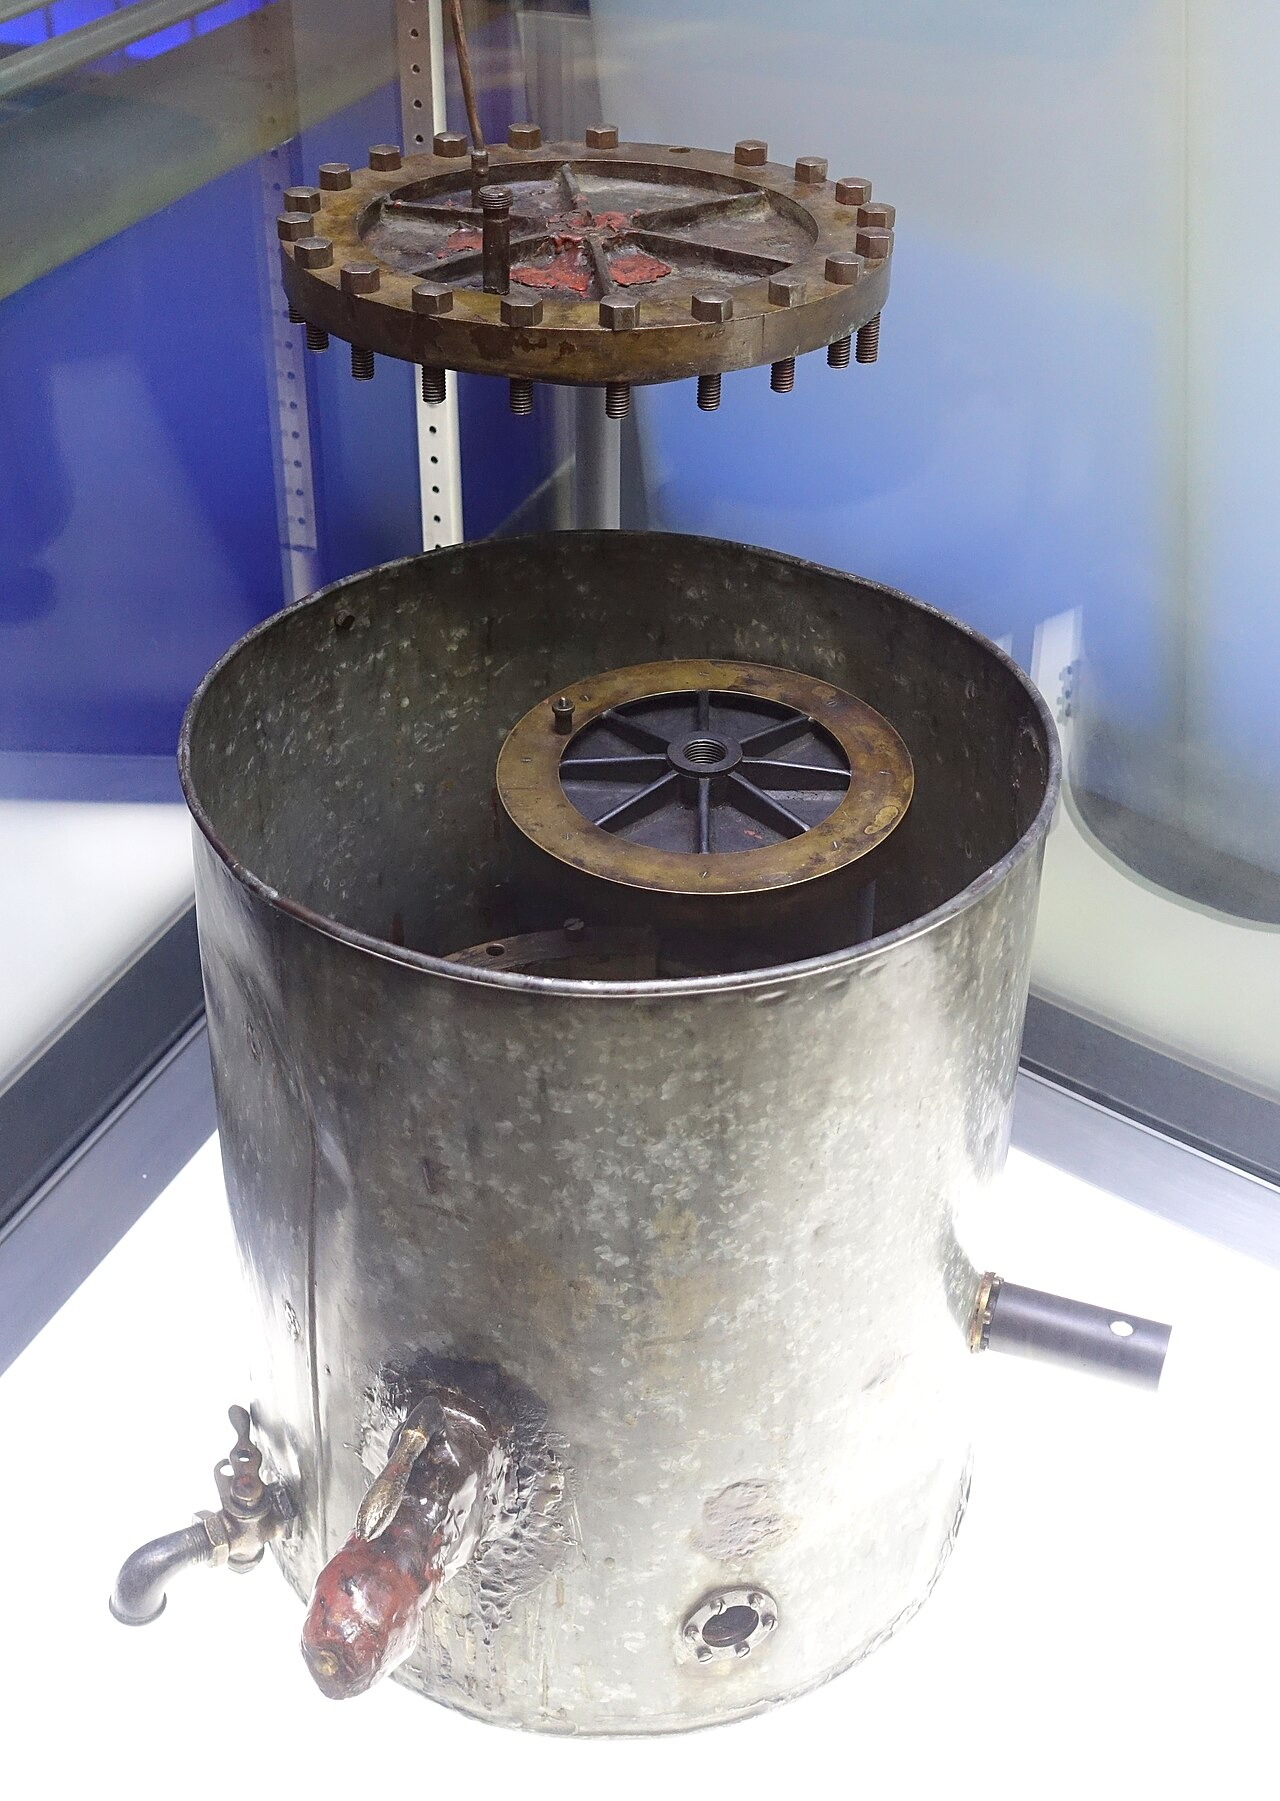
\includegraphics[width=0.36\linewidth]{images/book3/millikan-apparatus.jpg}

{\small L'appareil à gouttes d'huile de Millikan, vers 1916 (Museum of Science and Industry, Chicago)~: la chambre de laiton porte les deux armatures horizontales entre lesquelles on observait les gouttes.}
\end{omfigure}

\section{Problème~: la goutte d'huile de Millikan}

\begin{problem}[{Problème du week-end --- peser la charge de l'électron avec
une goutte d'huile~: Stokes, le condensateur plan, et un tableau de nombres
qui refusent d'être autre chose que des multiples d'un seul}]
\label{pb:b1:potential-capacitors:1}
On pulvérise des gouttes d'huile entre deux armatures horizontales distantes
de $d = \qty{16}{mm}$ et de \qty{20}{cm} de diamètre, que l'on observe au
\omterm{def:b1:optical-instruments:microscope}{microscope}. Données~: masse volumique de l'huile $\rho = \qty{900}{kg/m^3}$,
masse volumique de l'air \qty{1.2}{kg/m^3}, viscosité de l'air $\eta = \qty{1.8e-5}{Pa.s}$, $g =
\qty{9.8}{m/s^2}$, $\varepsilon_0 = \qty{8.85e-12}{F/m}$. Une petite sphère de
rayon $r$ animée de la vitesse $v$ dans l'air subit la force de Stokes $6\pi\eta rv$.

\medskip
\noindent\textbf{Partie I --- La goutte qui tombe.}
\begin{enumerate}
  \item Forces sur une goutte qui tombe sans tension appliquée~; montrer
        qu'elle atteint la \omterm{prop:b1:newton-dynamics:terminal}{vitesse limite} $v_1 = 2\rho gr^2/9\eta$ (on négligera
        la \omterm{thm:b1:fluid-statics:archimedes}{poussée d'Archimède} de l'air --- le justifier).
  \item Une goutte tombe de \qty{1.0}{mm} en \qty{10}{s}~: son rayon et sa masse.
  \item \omterm{def:b1:transient-regimes:firstorder}{Constante de temps} de l'approche de $v_1$~; distance parcourue
        pendant ce temps. Voit-on jamais la goutte accélérer~?
  \item Nombre de Reynolds $\rho_{\text{air}}v_1r/\eta$ du mouvement~: la \omterm{prop:b1:newton-dynamics:drag}{loi
        de Stokes} est-elle légitime~?
  \item Pourquoi les gouttes doivent-elles être si petites~? (Comparer le
        poids à la force électrique sur une \omterm{def:b1:electrostatics-gauss:charge}{charge élémentaire} dans un champ
        de \qty{3e5}{V/m}.)
  \item On voit la goutte trembler légèrement autour de sa chute moyenne~:
        qu'est-ce que c'est, et pourquoi cela limite-t-il la précision~?
\end{enumerate}

\medskip
\noindent\textbf{Partie II --- Le champ.}
On applique une tension $U$, l'armature supérieure étant positive.
\begin{enumerate}[resume]
  \item Champ entre les armatures pour $U = \qty{5.0}{kV}$~; pourquoi est-il
        uniforme, et quelles sont les équipotentielles~?
  \item \omterm{def:b1:potential-capacitors:capacitance}{Capacité} des armatures, charge qu'elles portent à \qty{5.0}{kV}, et
        énergie stockée.
  \item La goutte de la question~2 est immobilisée pour $U_0 = \qty{1080}{V}$~:
        signe et valeur de sa charge, en coulombs et en unités de $e$.
  \item Sous $U = \qty{5.0}{kV}$, la même goutte monte à la vitesse $v_2$~:
        montrer que $q = 6\pi\eta r(v_1 + v_2)d/U$ et calculer $v_2$.
  \item Pourquoi vaut-il mieux chronométrer une montée et une descente que
        chercher la tension d'équilibre~?
  \item \omterm{def:b1:work-and-energy:conservative}{Énergie potentielle} de la charge de la goutte entre les armatures sous
        \qty{5}{kV}, et énergie dissipée par la traînée pendant une montée de
        \qty{1}{cm}.
\end{enumerate}

\medskip
\noindent\textbf{Partie III --- Le tableau des charges.}
Exposée entre deux mesures à une faible source de rayons X, la même goutte
change de charge~; des mesures successives donnent (en $10^{-19}$~C)~:
$4.80$, $8.01$, $6.42$, $3.19$, $9.63$.
\begin{enumerate}[resume]
  \item Montrer que les cinq valeurs sont proches de multiples entiers d'une
        même quantité, et donner les entiers.
  \item Meilleure estimation de la \omterm{def:b1:electrostatics-gauss:charge}{charge élémentaire} à partir des cinq
        valeurs~; \omterm{def:b1:units-dimensions:uncertainty}{incertitude-type} sur la moyenne (\cref{ch:b1:units-dimensions}).
  \item Pourquoi la charge change-t-elle d'un nombre entier de $e$ d'une
        mesure à l'autre~?
  \item Montrer que, dans cette méthode, $q \propto \eta^{3/2}$~: de combien une
        erreur de $1\%$ sur la viscosité déplace-t-elle $e$~? (La valeur
        d'origine de Millikan était $0.6\%$ trop basse, précisément pour cette raison.)
  \item Les quarks portent $\pm e/3$ et $\pm 2e/3$~: pourquoi aucune goutte
        d'huile n'a-t-elle jamais montré un tiers de $e$~?
  \item La constante de Faraday, charge d'une \omterm{def:b1:kinetic-theory:scales}{mole} d'électrons, vaut
        $F = \qty{96485}{C/mol}$~: en déduire le nombre d'Avogadro.
  \item Thomson avait mesuré $e/m_e = \qty{1.76e11}{C/kg}$ pour l'électron~:
        en déduire sa masse, et la comparer à celle d'un atome d'hydrogène
        (\qty{1.67e-27}{kg}).
\end{enumerate}

\medskip
\noindent\textbf{Partie IV --- L'appareil, vu par le potentiel.}
\begin{enumerate}[resume]
  \item Esquisser les équipotentielles et les \omterm{def:b1:electrostatics-gauss:field}{lignes de champ} entre les
        armatures, effets de bord compris~; justifier qu'on les néglige.
  \item Une goutte chargée positivement à la hauteur $z$ au-dessus de
        l'armature inférieure (portée à \qty{0}{V})~: \omterm{def:b1:work-and-energy:conservative}{énergie potentielle} en
        fonction de $z$~; \omterm{def:b1:work-and-energy:conservative}{énergie potentielle} totale en comptant la
        pesanteur~; condition sur $U$ pour le point d'équilibre.
  \item Comparer l'énergie de la charge de la goutte (question~12) à
        l'énergie stockée dans le \omterm{def:b1:potential-capacitors:capacitance}{condensateur}~: la goutte perturbe-t-elle le
        champ~?
  \item On inverse la tension (armature inférieure positive) avec
        $U = \qty{5.0}{kV}$~: que fait la goutte de la question~9, et à quelle
        vitesse~?
  \item Un grain de poussière de \qty{1}{\micro g} portant $10^4e$ dans le
        même champ~: rapport de la force électrique au poids~; pourquoi de
        tels grains ne peuvent pas être maintenus en lévitation, et pourquoi
        Millikan a choisi un brouillard d'huile.
  \item Récapituler~: qu'a-t-on mesuré (trois fois), qu'en a-t-on déduit, avec
        quelle incertitude, et quelles deux constantes en ont découlé.
\end{enumerate}
\end{problem}
